
\section{Снижение дисперсии с помощью контрольных переменных}
\subsection{Пример}

\begin{frame}{Президентские выборы во Франции 2012 \parencite{pons2018will}}
\begin{columns}
\begin{column}{0.5\textwidth}
    
   \begin{center}
   Франсуа Олланд
   \vskip1em
     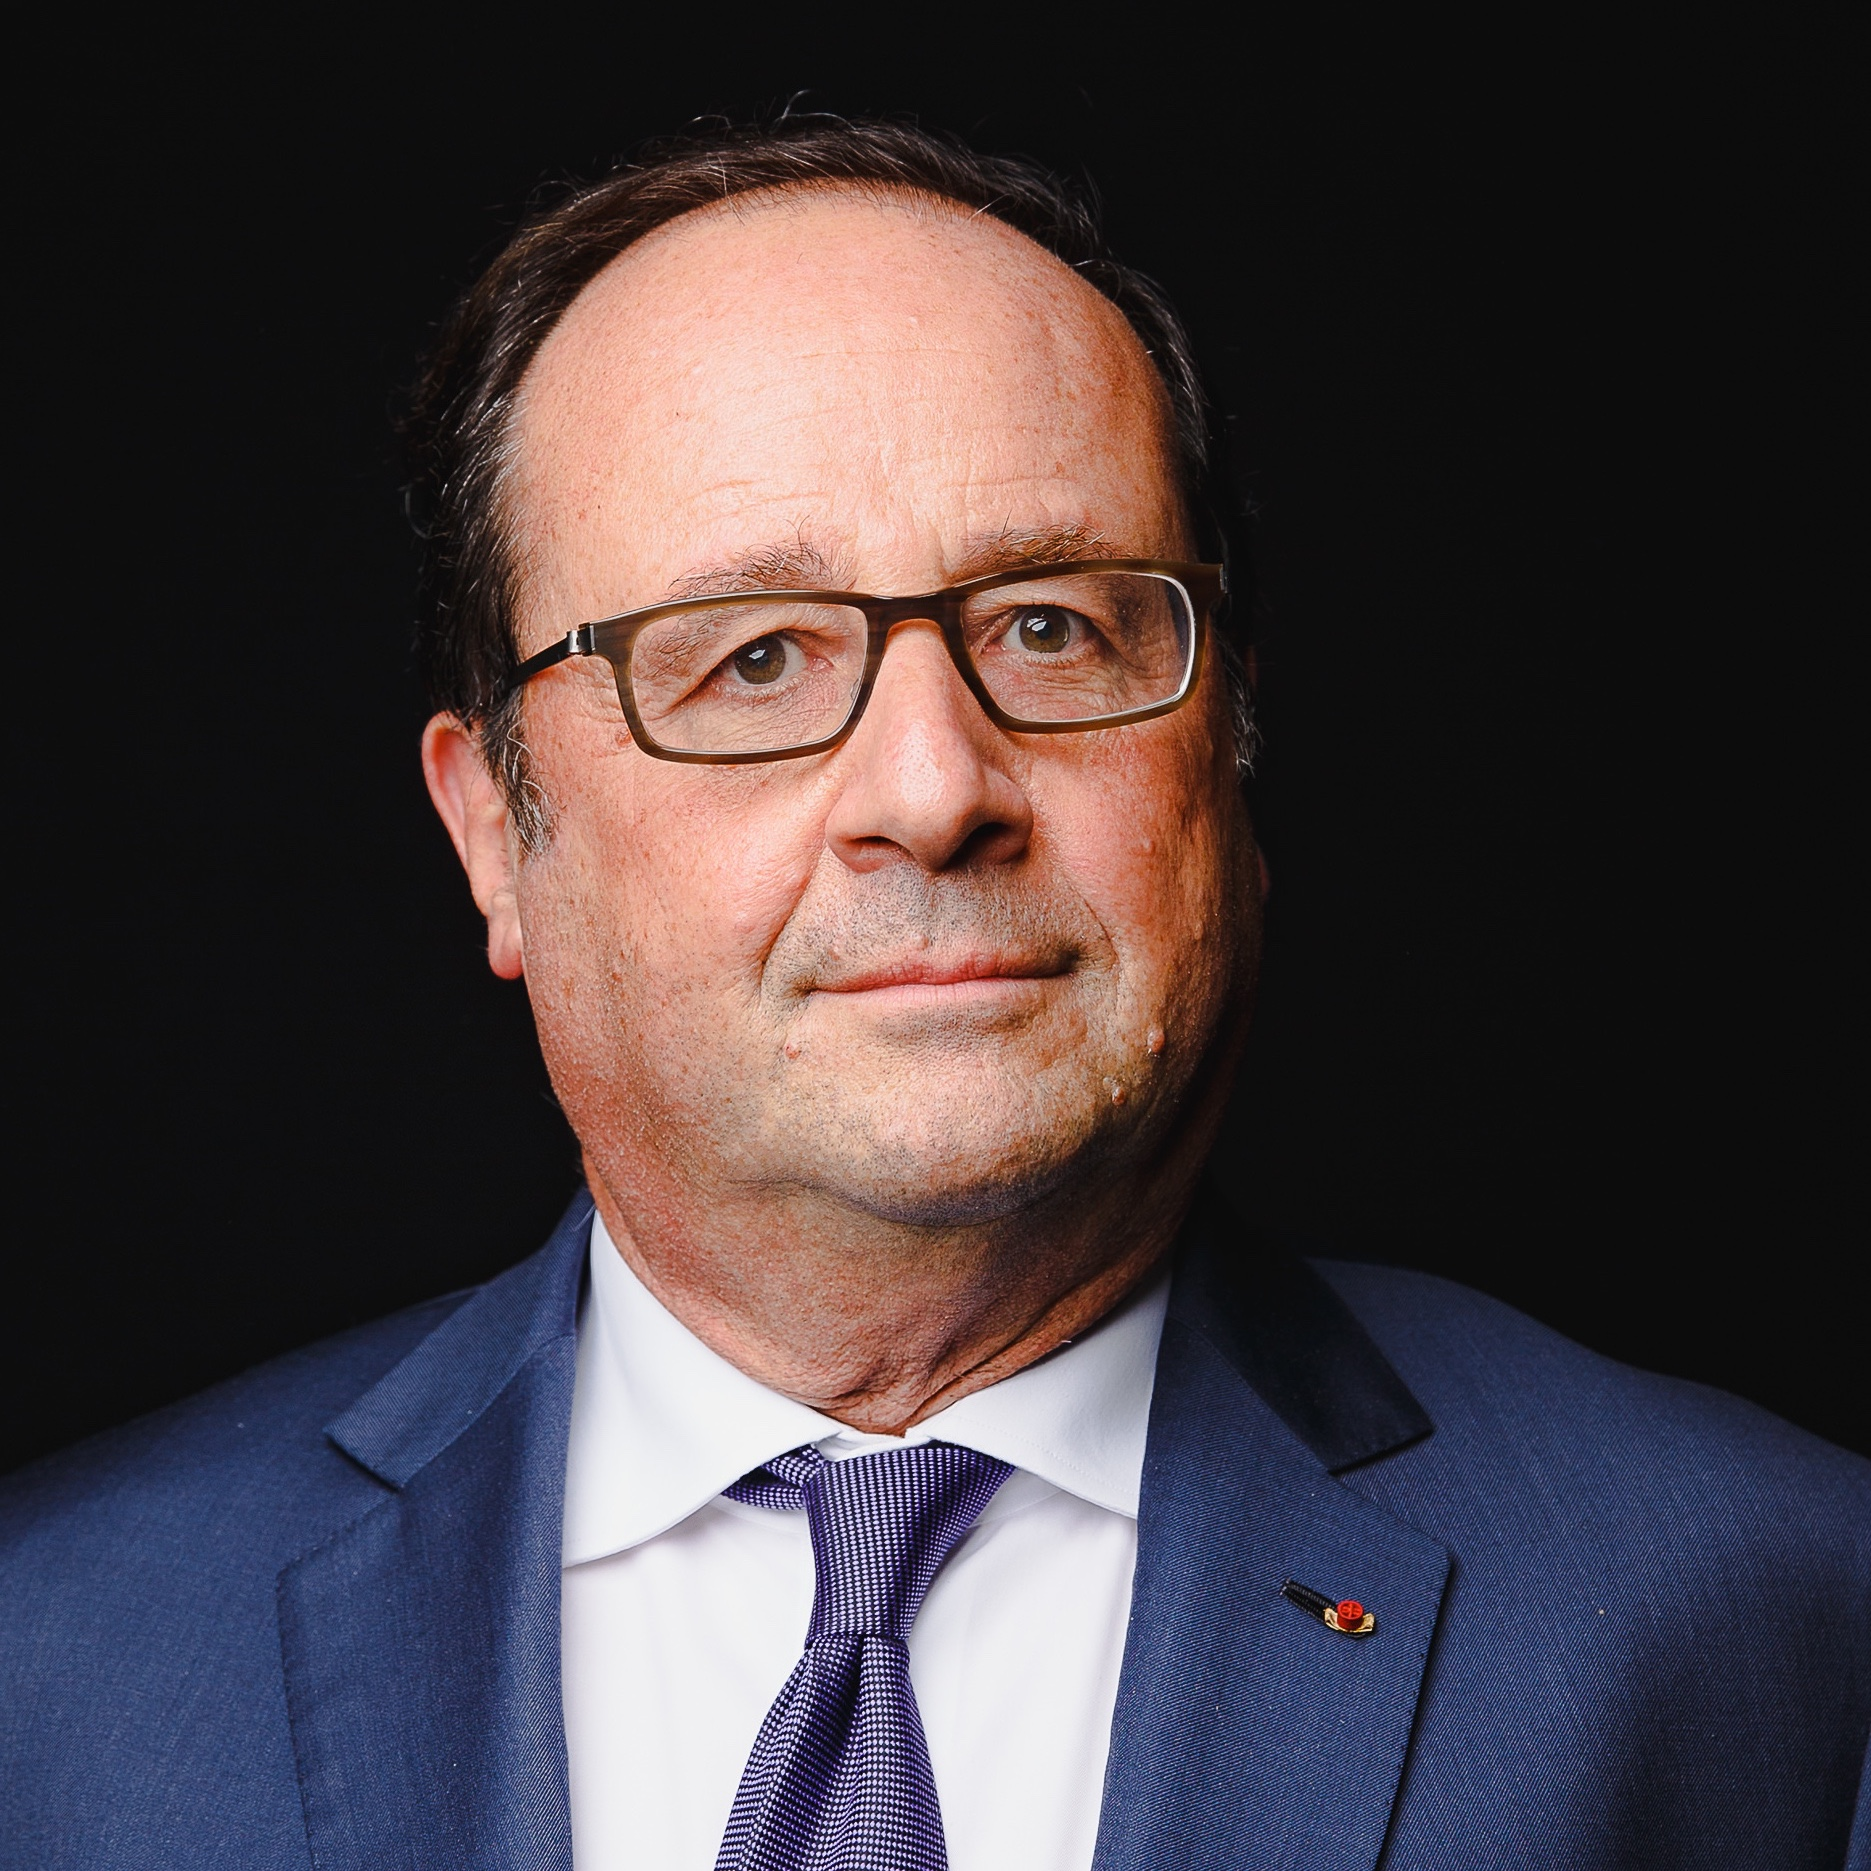
\includegraphics[width=0.8\textwidth]{Images/hollande.jpg}
     \vskip1em
     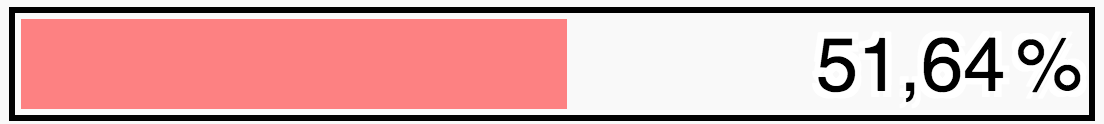
\includegraphics[width=0.8\textwidth]{Images/hollande_votes.png}
     \end{center}
     
\end{column}
\begin{column}{0.5\textwidth} 
    
    \begin{center}
    Николя Саркози
    \vskip1em
     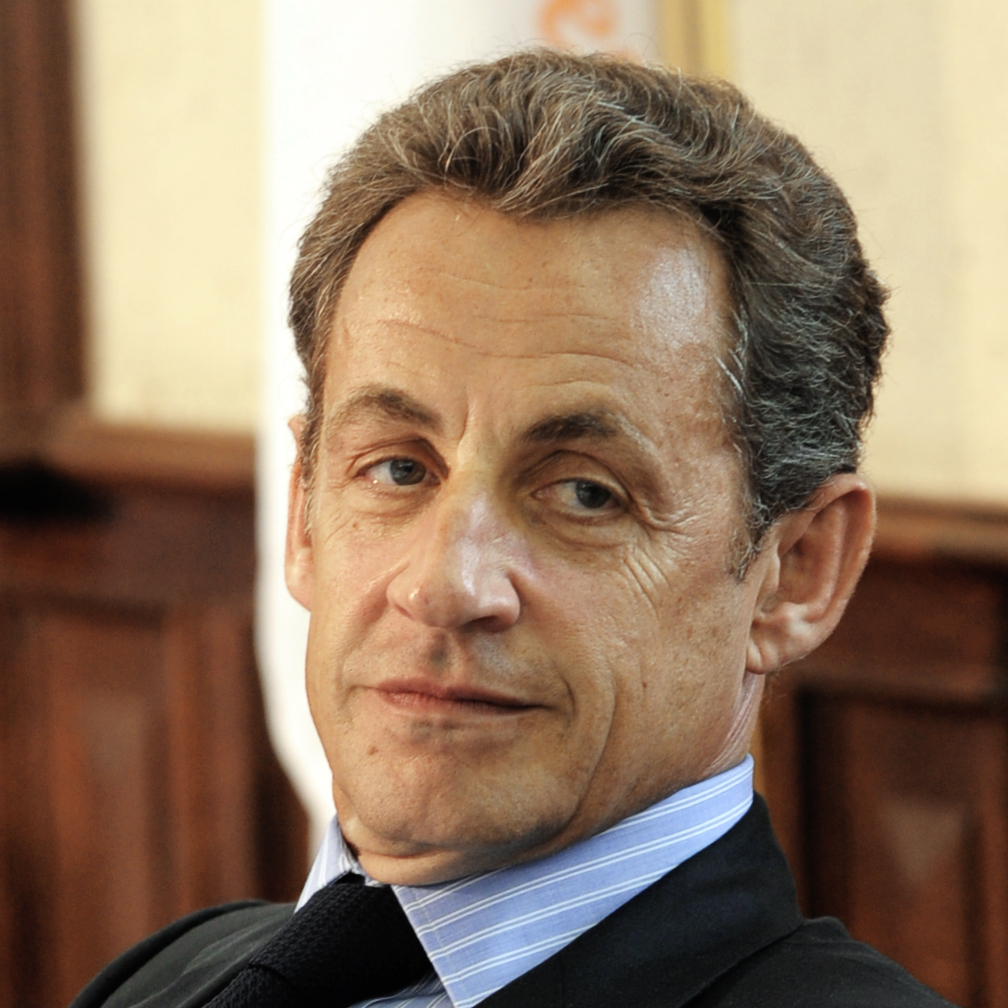
\includegraphics[width=0.8\textwidth]{Images/sarkozy.jpg}
     \vskip1em
     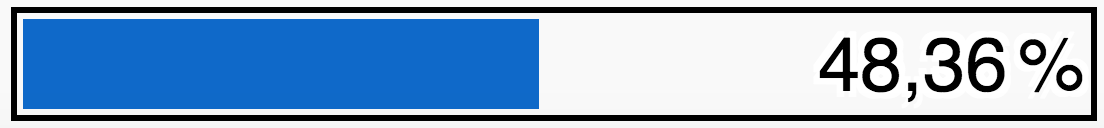
\includegraphics[width=0.8\textwidth]{Images/sarkozy_votes.png}
     \end{center}
\end{column}
\end{columns}
\end{frame}

\begin{frame}{Президентские выборы во Франции 2012 \parencite{pons2018will}}
\begin{columns}
\begin{column}{0.5\textwidth}
    
   \begin{center}
   Франсуа Олланд
   \vskip1em
     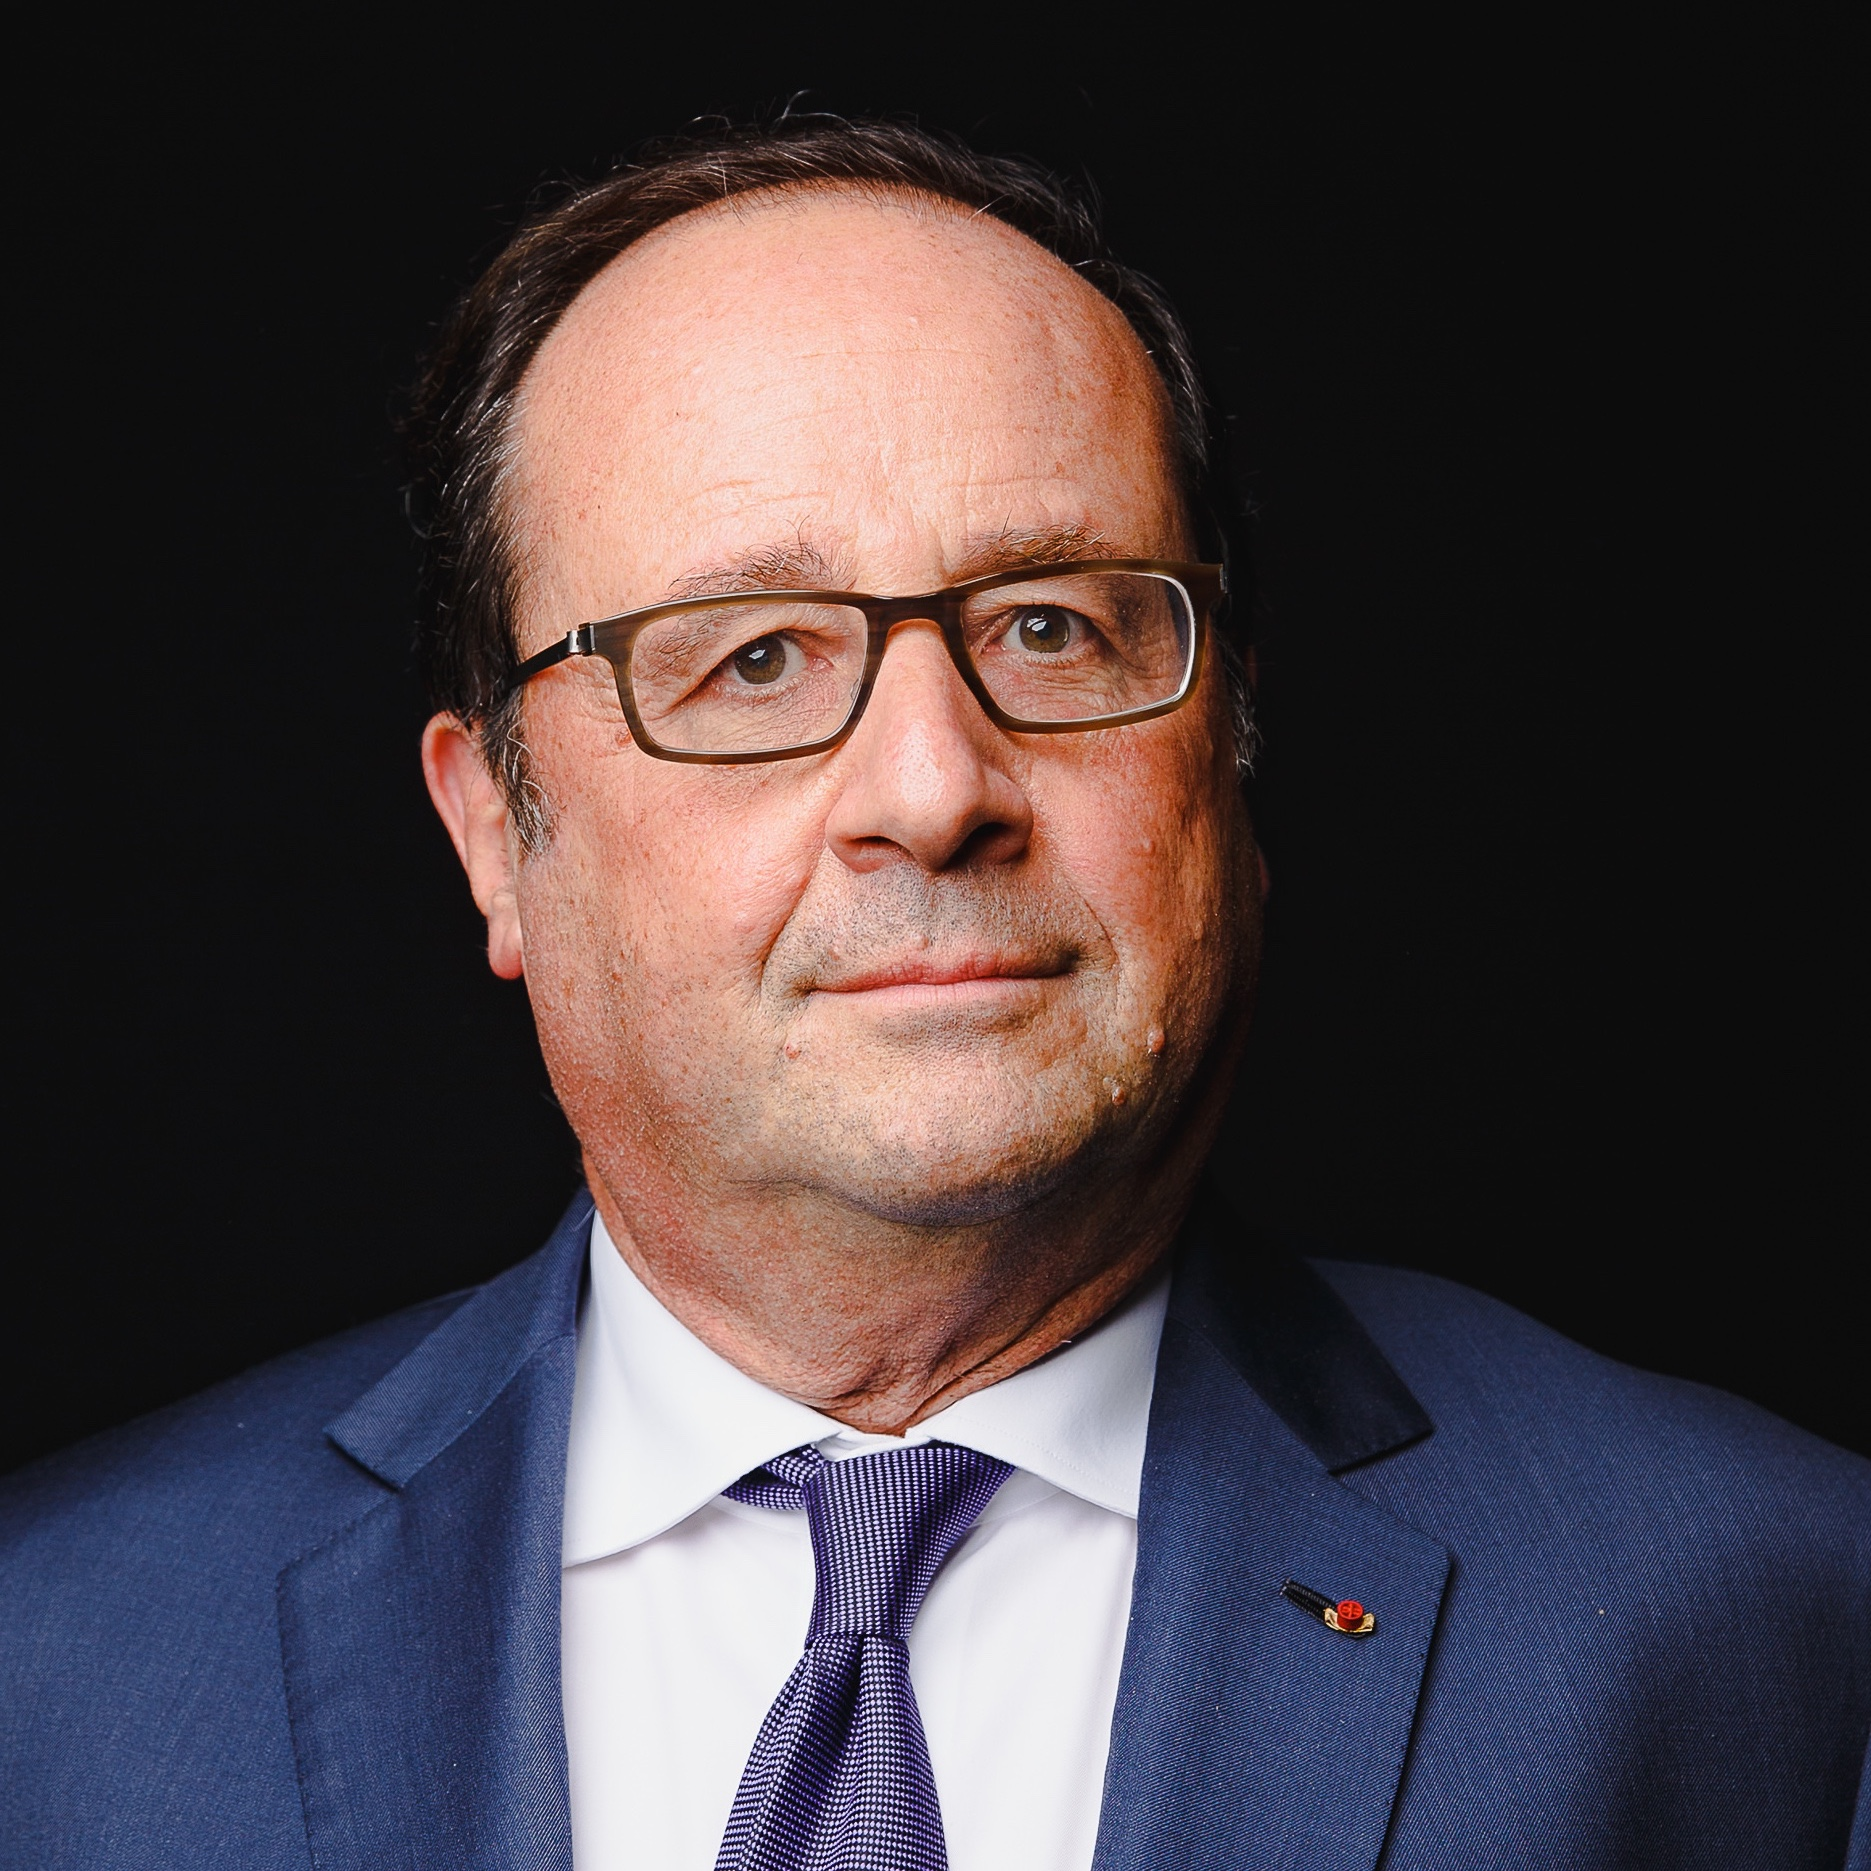
\includegraphics[width=0.8\textwidth]{Images/hollande.jpg}
     \vskip1em
     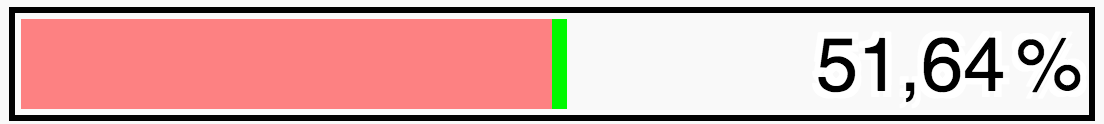
\includegraphics[width=0.8\textwidth]{Images/hollande_effect.png}
     \end{center}
\end{column}
\begin{column}{0.5\textwidth} 
    
    \begin{center}
    Николя Саркози
    \vskip1em
     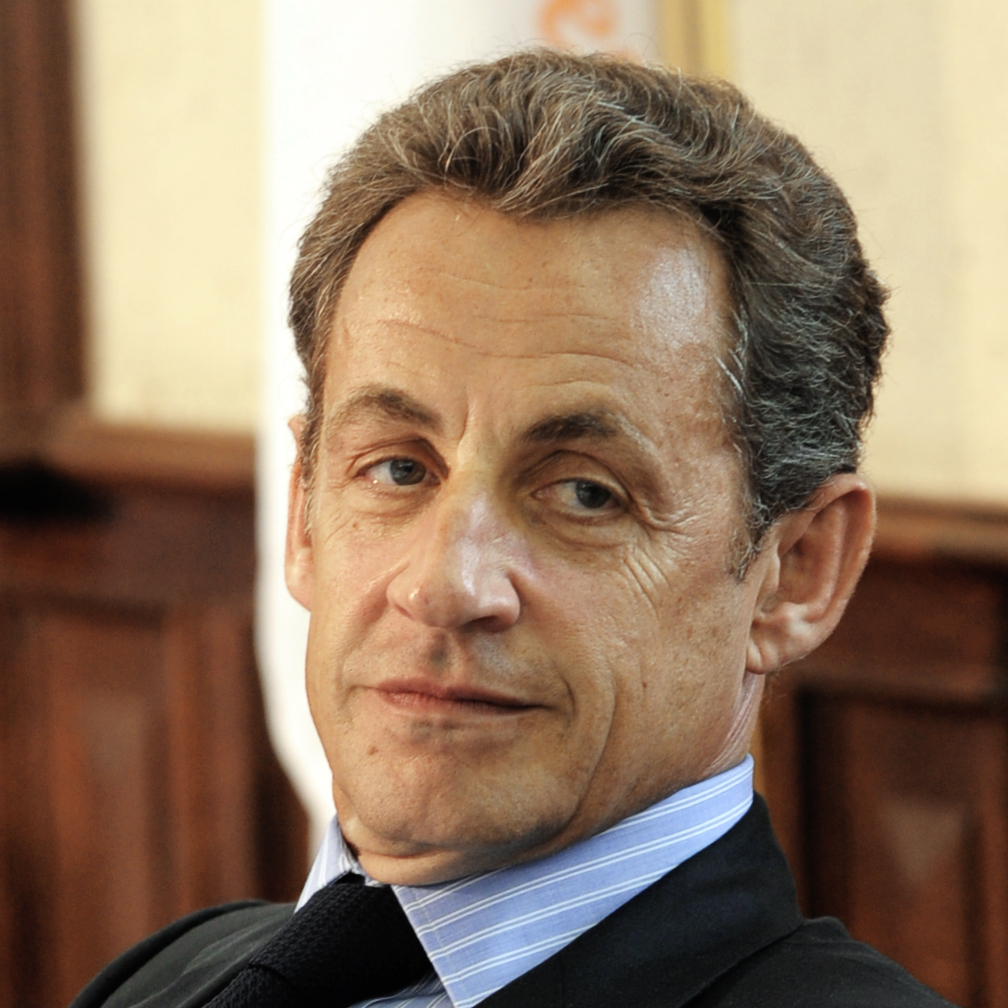
\includegraphics[width=0.8\textwidth]{Images/sarkozy.jpg}
     \vskip1em
     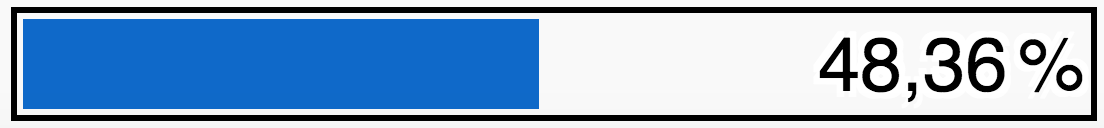
\includegraphics[width=0.8\textwidth]{Images/sarkozy_votes.png}
     \end{center}
\end{column}
\end{columns}
Эффект от агитации в 0.5 процентных пункта. 
\end{frame}

\begin{frame}{Как суметь поймать такой эффект?}

2 метода снижения дисперсии:
\begin{enumerate}
    \item Контрольные переменные \textbf{(covariates)}
    \item Грамотное планирование эксперимента и престратификация (в другой раз)
\end{enumerate}
    
\end{frame}

\subsection{Ковариаты}

\begin{frame}{Ковариаты\footnote{\cite[Раздел 3.1.1]{angrist2008mostly}, \cite[Глава 7.5-7.8]{imbens2015causal}}}
    \begin{itemize}
    \item $Y_1$, $Y_0$ -- потенциальные исходы (\textbf{potential outcomes})
    \item $T$ -- 1, если наблюдение в эксперименте и 0 иначе (\textbf{treatment variable})
    \item $X$ -- Независимые переменные (\textbf{covariates})
\end{itemize}
% спросить вспомнить предпосылку
\pause
Ковариаты $X$ меняются  вместе с $Y_1$ и $Y_0$ (\textbf{ковариируют} или (мульти) \textbf{коррелируют})

$$\mathbb{C}\text{ov}(X, Y_1) > 0, \mathbb{C}\text{ov}(X, Y_0) > 0$$

\end{frame}

\begin{frame}{Маленький пример}
\begin{table}[]
\begin{tabular}{l|l|l||l}
&$Y_1$ & $Y_0$ & X \\
\hline
Пациент 1 & - & 36.6 & Из Европы \\
Пациент 2 & 36.6   & - & Из Европы \\
Пациент 3 & 35 & -  &  Из Европы \\
Пациент 4 & - & 36 &  Из Европы \\
Пациент 5 & 37.3   & - &  Из Азии \\
Пациент 6 & - & 39.3 &  Из Азии \\
Пациент 7 & 37.2   & - &  Из Азии \\
Пациент 8 & - & 39.2 &  Из Азии
\end{tabular}
\end{table}
\begin{itemize}[<+->]
    \item \textit{Повторение}. На глаз. Выполнена ли предпосылка экзогенности? $(Y_1, Y_0, X)_i \perp T_i$
    \item Высока ли дисперсия с одним и тем же $X$: $\mathbb{V}(Y|X)$? 
    \item У кого в среднем выше температура? $\mathbb{C}\text{ov}(X, Y_0)$ -- ?
    \item Высока ли общая дисперсия: $\mathbb{V}(Y)$? 
\end{itemize}

\end{frame}

\begin{frame}{То же, но на картинке}
\begin{figure}
    \centering
    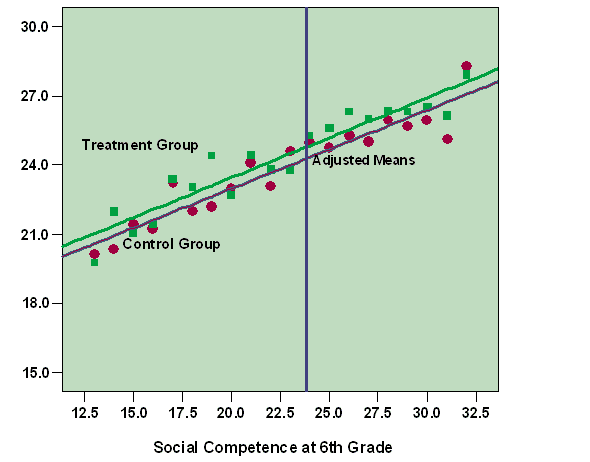
\includegraphics[width=\textwidth]{Images/covariates.png}
\end{figure}
\end{frame}


\begin{frame}{Контроль, снижающий дисперсию}

\begin{gather*}
    \mathbb{V}(Y) = \mathbb{E}\left((Y - \mathbb{E}Y)^2\right) = \\
    \mathbb{E}\left(\left(Y - \mathbb{E}(Y|X) + \mathbb{E}(Y|X) - \mathbb{E}Y\right)^2\right) = \\
    \mathbb{E}\left((Y - \mathbb{E}(Y|X))^2\right) + \mathbb{E}\left((\mathbb{E}(Y|X) - \mathbb{E}Y)^2\right) +
    \\2\mathbb{E}\left(\left(\mathbb{E}(Y|X) - \mathbb{E}Y\right)\left(Y - \mathbb{E}(Y|X)\right)\right) = \\
    \mathbb{E}(\mathbb{V}(Y|X)) + \mathbb{V}(\mathbb{E}(Y|X)) + 0
\end{gather*} 
\end{frame}


\begin{frame}{Результаты выборов во Франции}
\begin{figure}
    \centering
    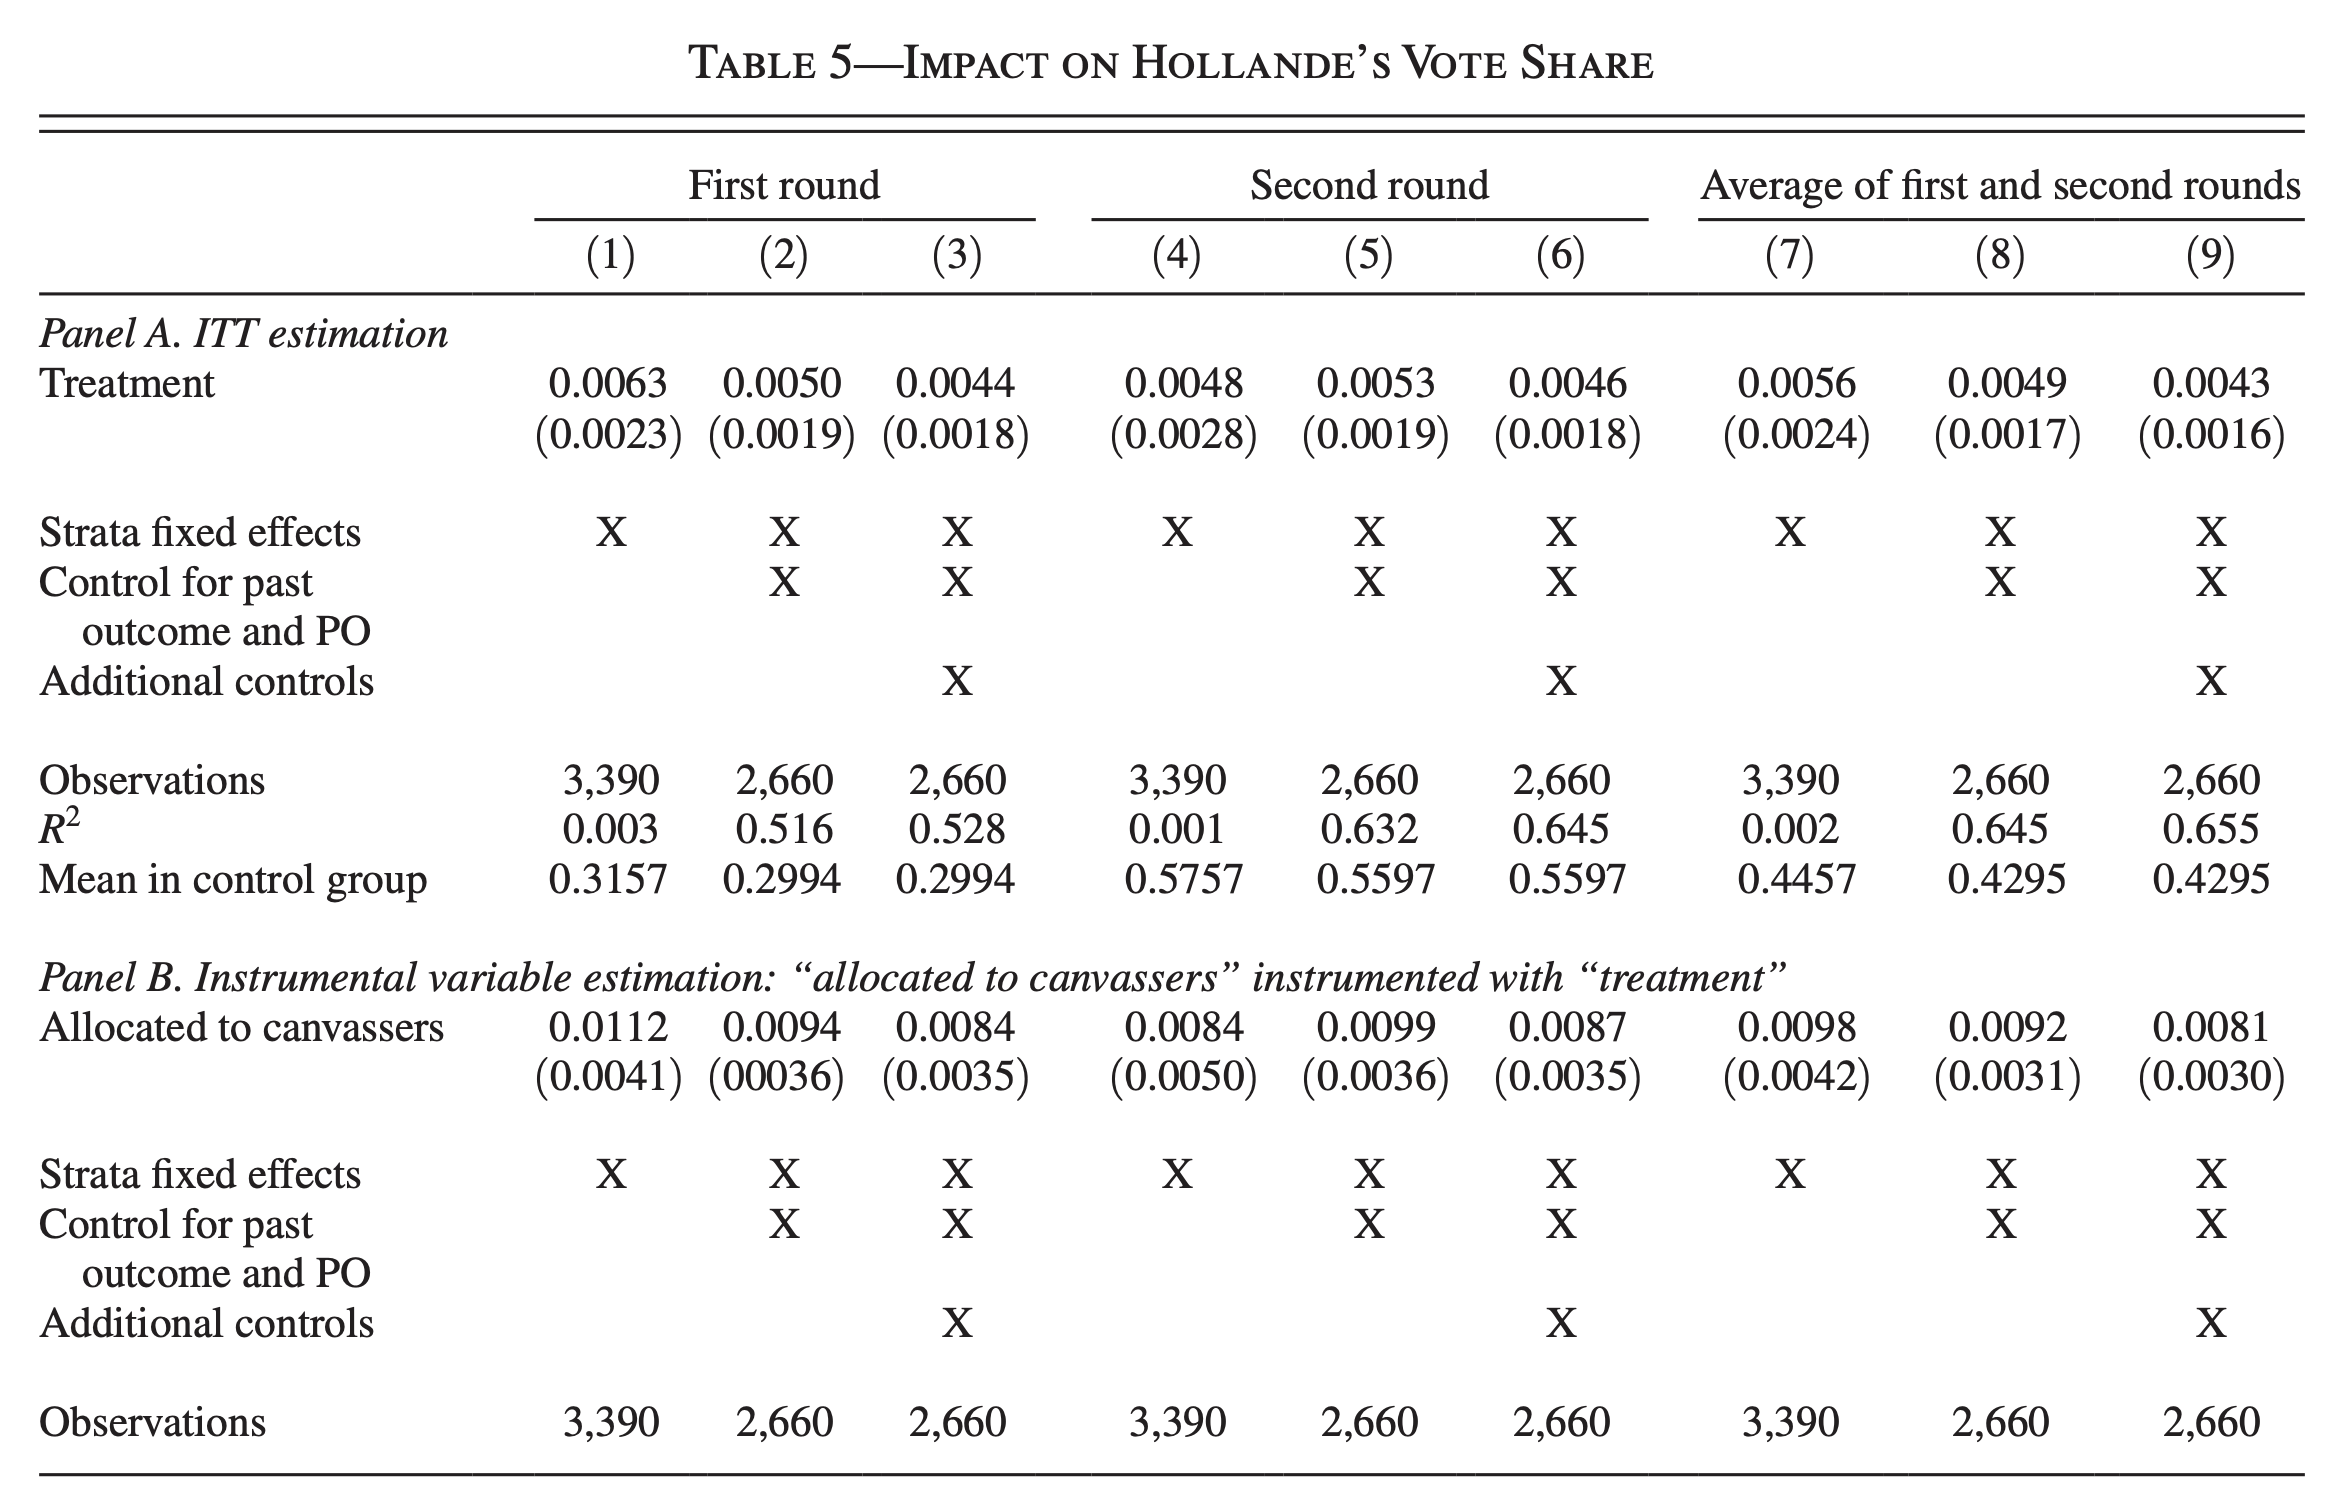
\includegraphics[width=\textwidth]{Images/pons_table.png}
\end{figure}
\end{frame}


\begin{frame}{Повторение. А это зачем?}
\begin{figure}
    \centering
    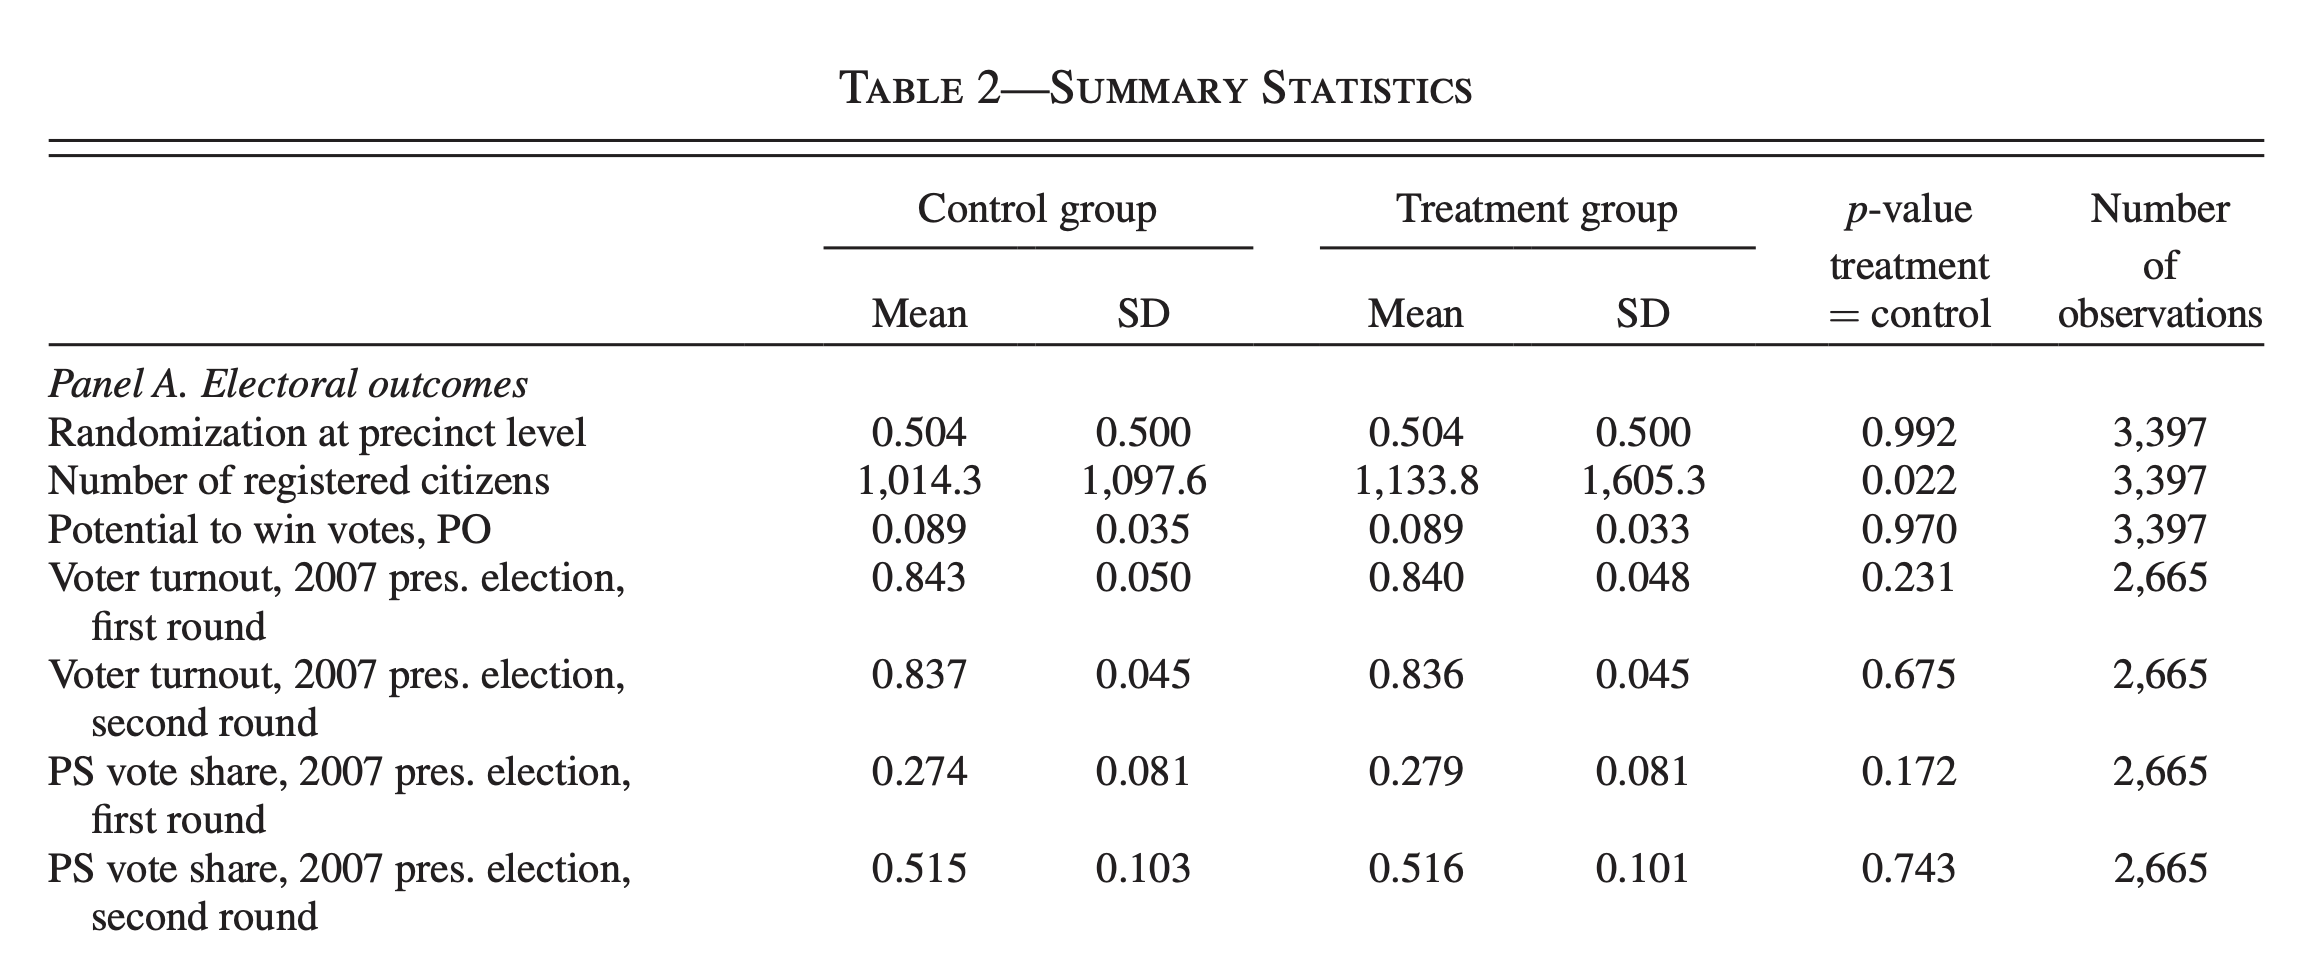
\includegraphics[width=\textwidth]{Images/balance.png}
\end{figure}
\end{frame}

\begin{frame}{Повторение. А это зачем?}
\begin{figure}
    \centering
    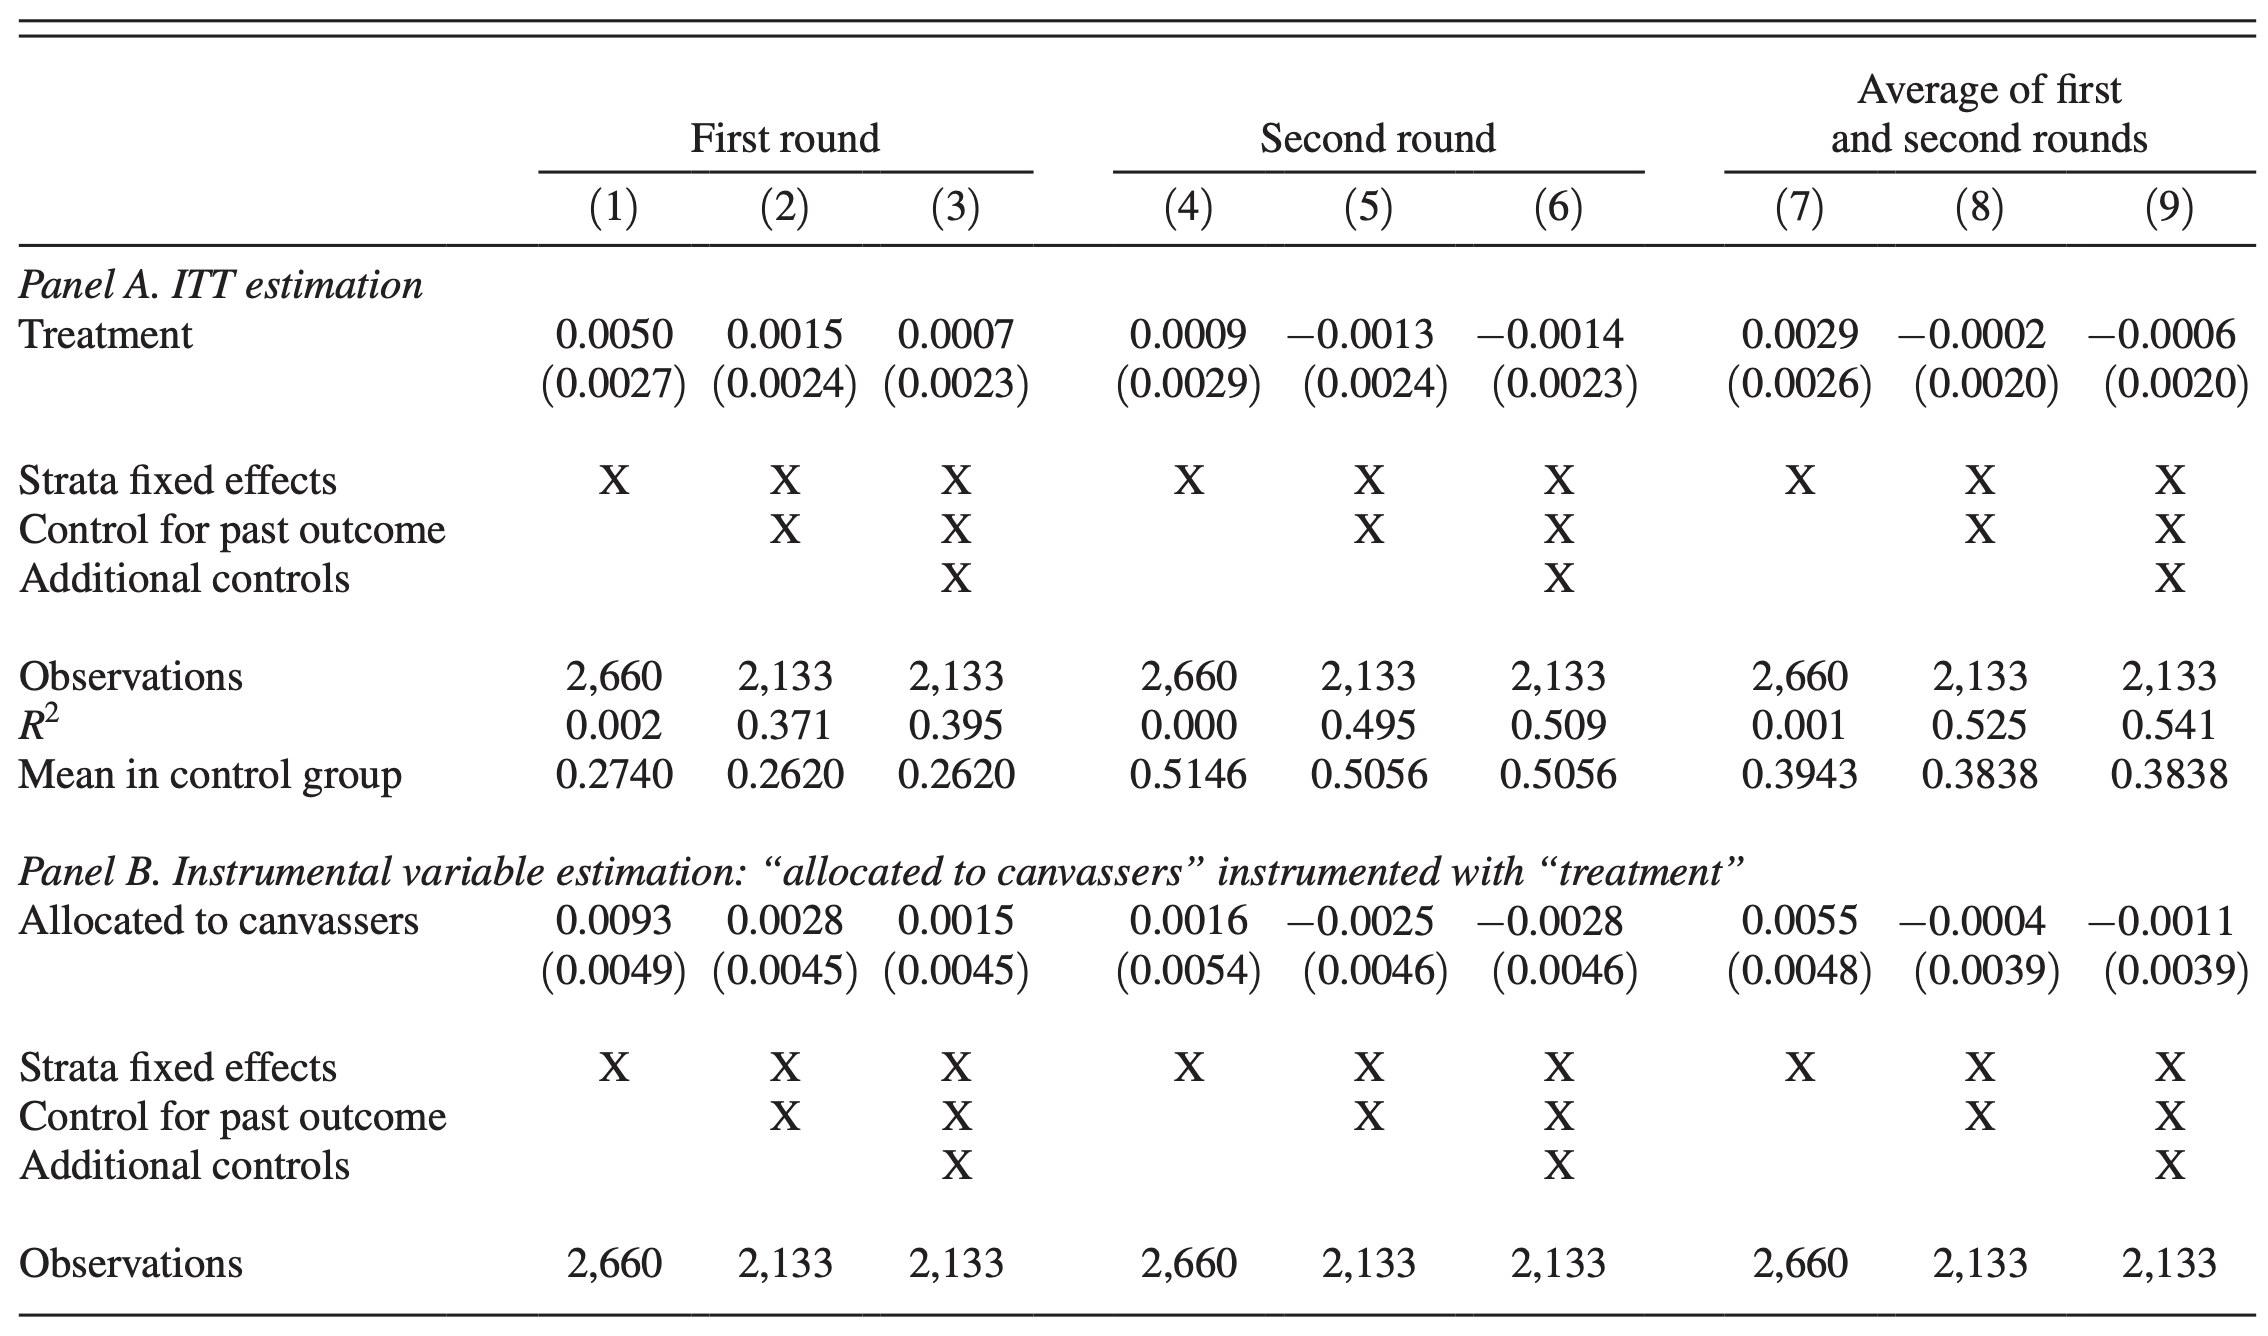
\includegraphics[width=\textwidth]{Images/palcebo.png}
\end{figure}
\end{frame}